\chapter{Motivation}\label{sec-motivation}

Satellites in orbit around Earth are used in many areas and disciplines, including space science, Earth observation, meteorology, climate research, telecommunication, navigation and human space exploration. They offer a unique resource for collecting scientific data, commercial opportunities and various essential applications and services, which lead to unrivalled possibilities for research and exploitation.

However, in the past decades, with increasing space activities, a new and unexpected hazard has started to emerge: space debris.

\begin{figure}[ht]
\centering
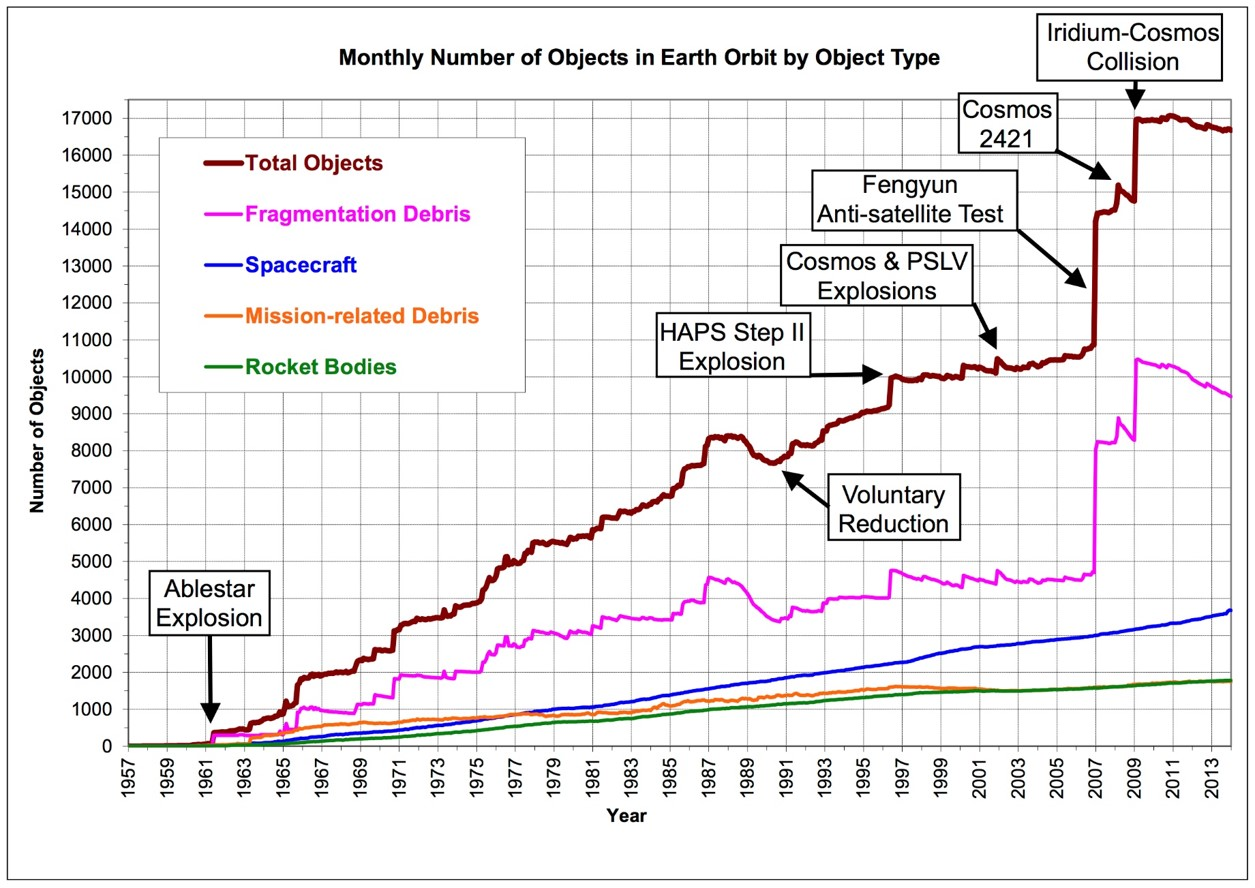
\includegraphics[width=1\textwidth]{fig/motivation/CataloguedSpaceDebrisOverTime}
\caption{Catalogued space debris over time}\cite{wright2010current}
\label{moti-CataloguedSpaceDebrisOverTime}
\end{figure}

The Figure \ref{moti-CataloguedSpaceDebrisOverTime} showes the debris changing trend over nearly 60 years. The y direction shows the number of objects. Each point represents the monthly numberof objects in Earth Orbit. The x direction is time axis. Space debris is divided into four types, each type has its own color: 
\begin{enumerate}
\item{Fragmentation Debris}
\item{Spacecraft}
\item{Mission-related Debris}
\item{Rocket Bodies}
\end{enumerate}


The orbris increasing of Spacecraft and Rocket Bodies are quite linearly. Mission-related Debris is quite stable. The most dramatic changing type is Fragmentation Drbis and this type of debris is directly related to satellite explosion and artificial celestial body collision.


From another statistical result \cite{}, we can see this trend much more clearly. In almost 60 years of space activities, more than 5250 launches have resulted in some 42 000 tracked objects in orbit, of which about 23000 remain in space and are regularly tracked by the US Space Surveillance Network and maintained in their catalogue, which covers objects larger than about 5–10 cm in low-Earth orbit (LEO) and 30 cm to 1 m at geostationary (GEO) altitudes. Only a small fraction – about 1200 – are intact, operational satellites today.

This large amount of space hardware has a total mass of more than 7500 tonnes.

\begin{figure}[ht]
\centering
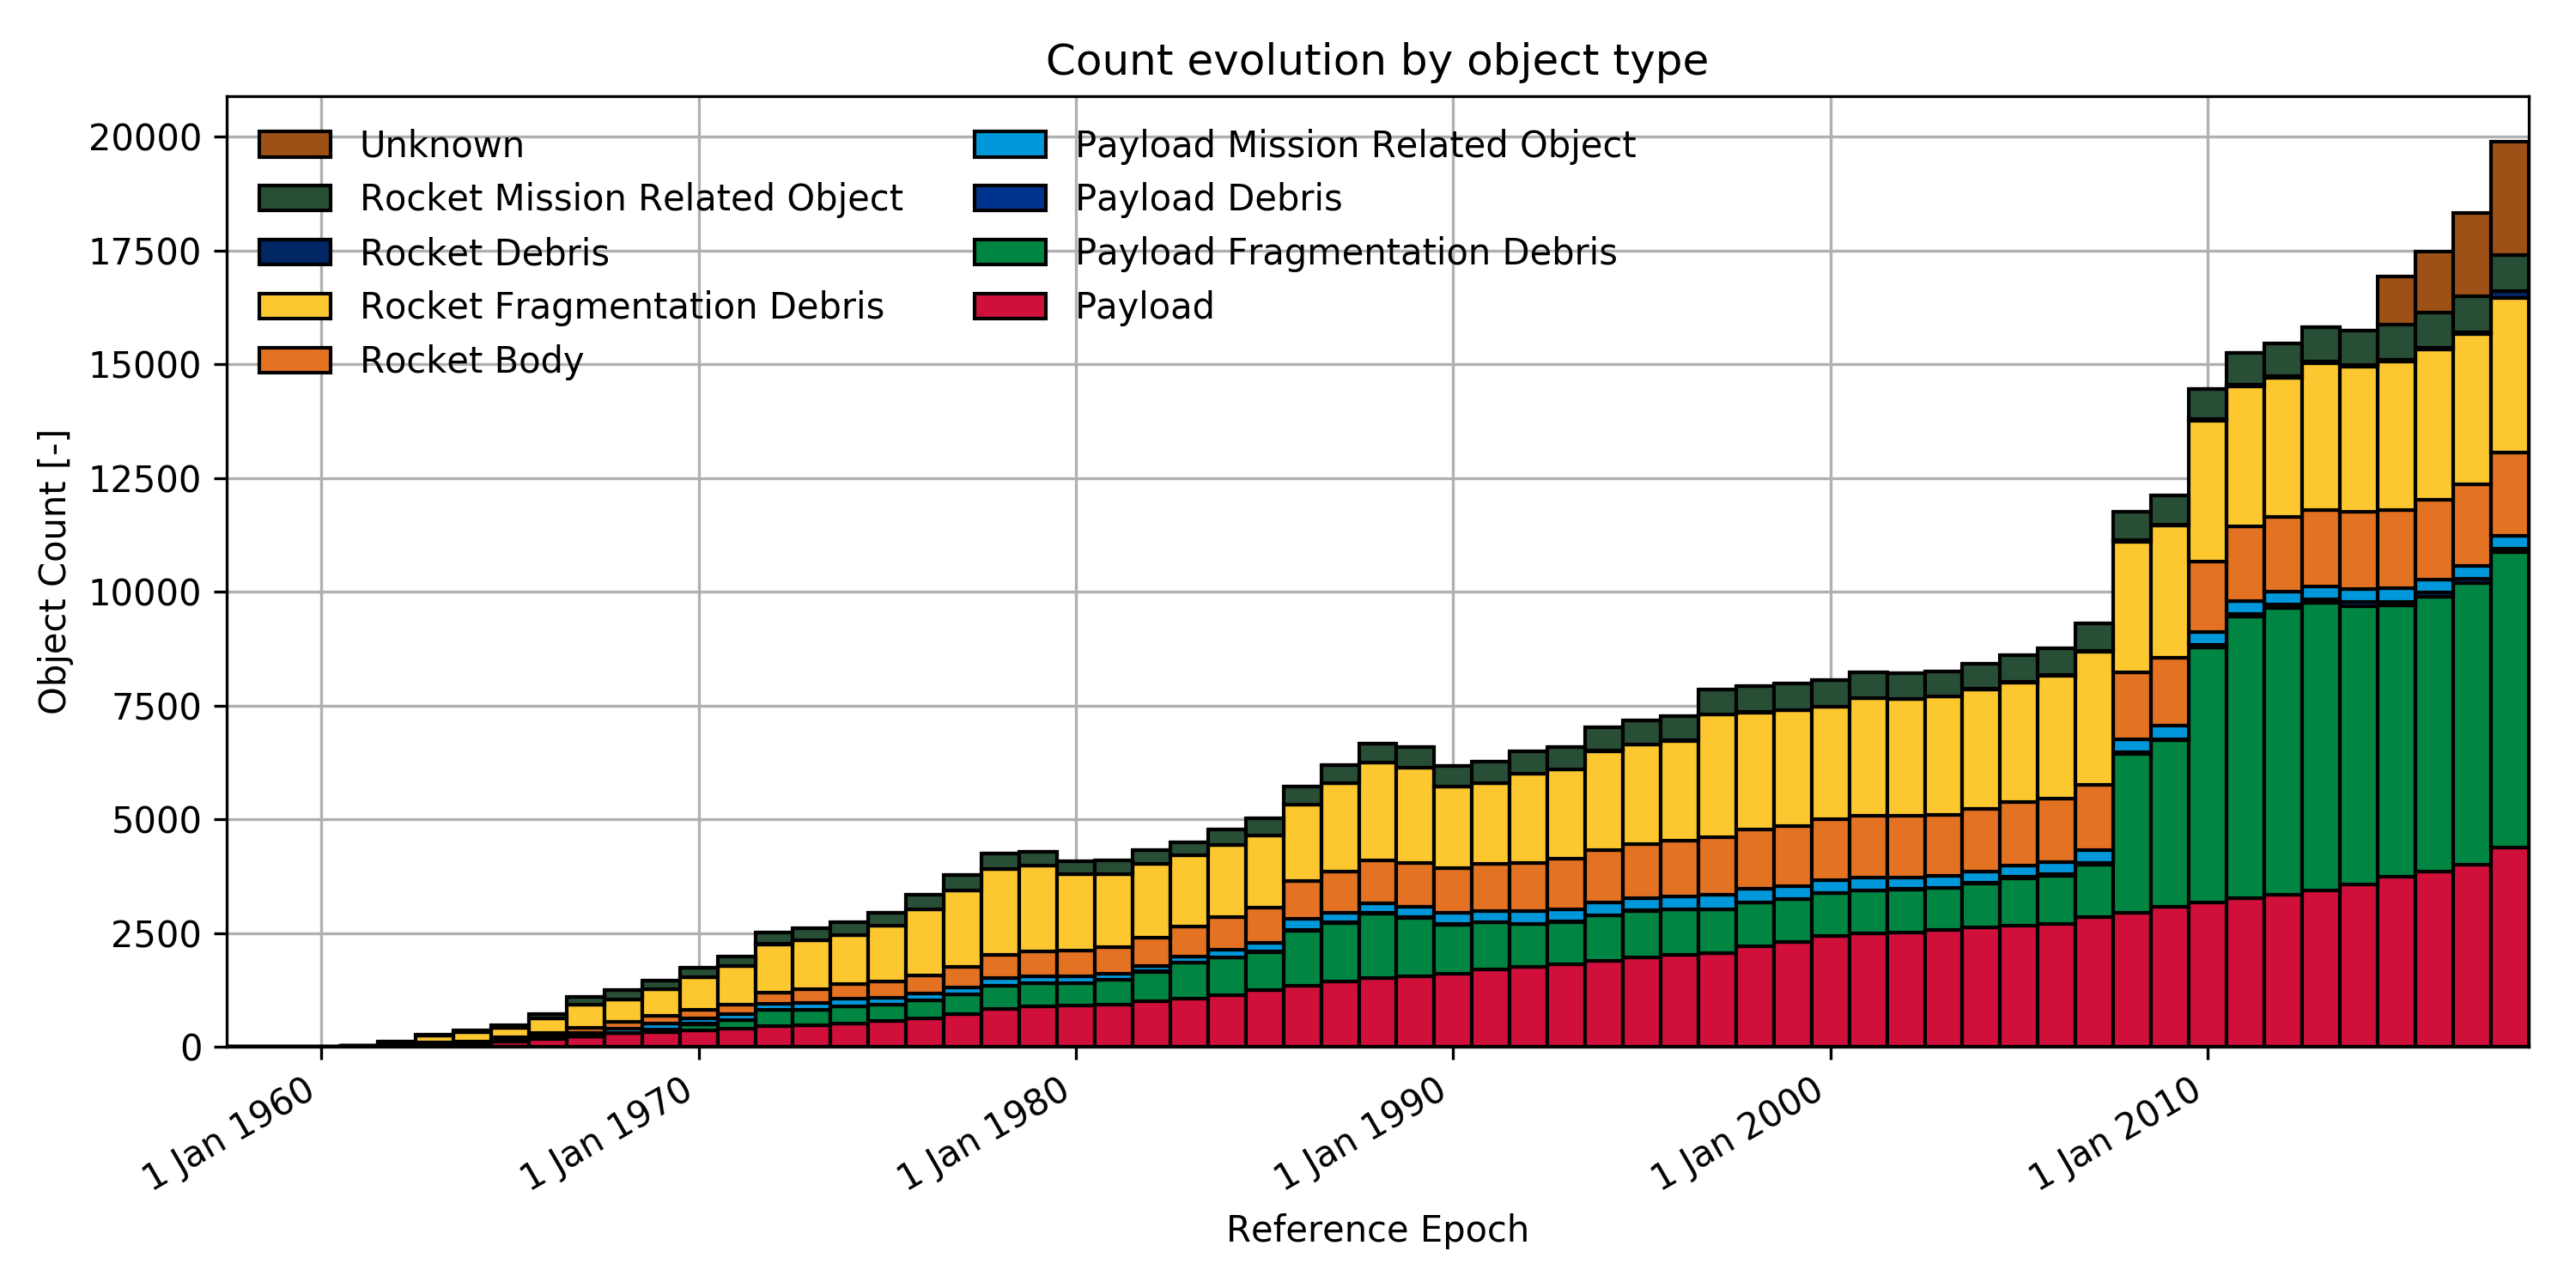
\includegraphics[width=\textwidth]{fig/motivation/all_evo_type_count}
\caption{Conut evolution by object type}
\label{moti-all_evo_type_count}
\end{figure}

\begin{enumerate}
\item{Spent upper stages}\\
About 24\% of the catalogued objects are satellites (less than a third of which are operational), and about 18\% are spent upper stages and mission related objects such as launch adapters and lens covers.

More than 290 inorbit fragmentation events have been recorded since 1961. Only a few were collisions and the majority of the events were explosions of spacecraft and upper stages.

\item{Explosions of satellites and rocket bodies}\\
These fragmentation events are assumed to have generated a population of objects larger than 1 cm numbering on the order of 750000. The sporadic flux from naturally occurring meteoroids may only prevail over that from human-made debris objects near sizes of 0.1-1 mm.

The main cause of inorbit explosions is related to residual fuel that remains in tanks or fuel lines, or other remaining energy sources, that remain on board once a rocket stage or satellite has been discarded in Earth orbit.

Over time, the harsh space environment can reduce the mechanical integrity of external and internal parts, leading to leaks and/or mixing of fuel components, which could trigger self-ignition. The resulting explosion can destroy the object and spread its mass across numerous fragments with a wide spectrum of masses and imparted velocities.

\item{Antisagellite test}\\
Besides such accidental break-ups, satellite interceptions by surface-launched missiles have been a major contributor in the recent past.

The Chinese FengYun-1C engagement in January 2007 alone increased the trackable space object population by 25\%.
\item{Other sources}\\
Solid rocket-motor firings, the ejection of reactor cores from Buk reactors after the end of operation of Russian radar ocean reconnaissance satellites in the 1980s and the relase of thin copper wires as part of a radio communication experiment during the Midas missions in the 1960s are the three most important sources.
\end{enumerate}

The nightmare scenario that space debris experts contemplate is called the Kessler syndrome, after American astrophysicist Donald Kessler. In 1978, while working for NASA, he published an analysis\cite{kessler1978collision} that showed frequent collisions exponentially increased the amount of space debris, leading to many more collisions, leading to much more debris until we lose the use of certain orbits because anything we put there would certainly be hit.

\begin{quote}
\em{"Since 2002, The growth has entered into the more feared exponential trend."}
\end{quote}
There can be absolutely no doubt that the time to do something about space debris has arrived.

\begin{figure}[ht]
\centering
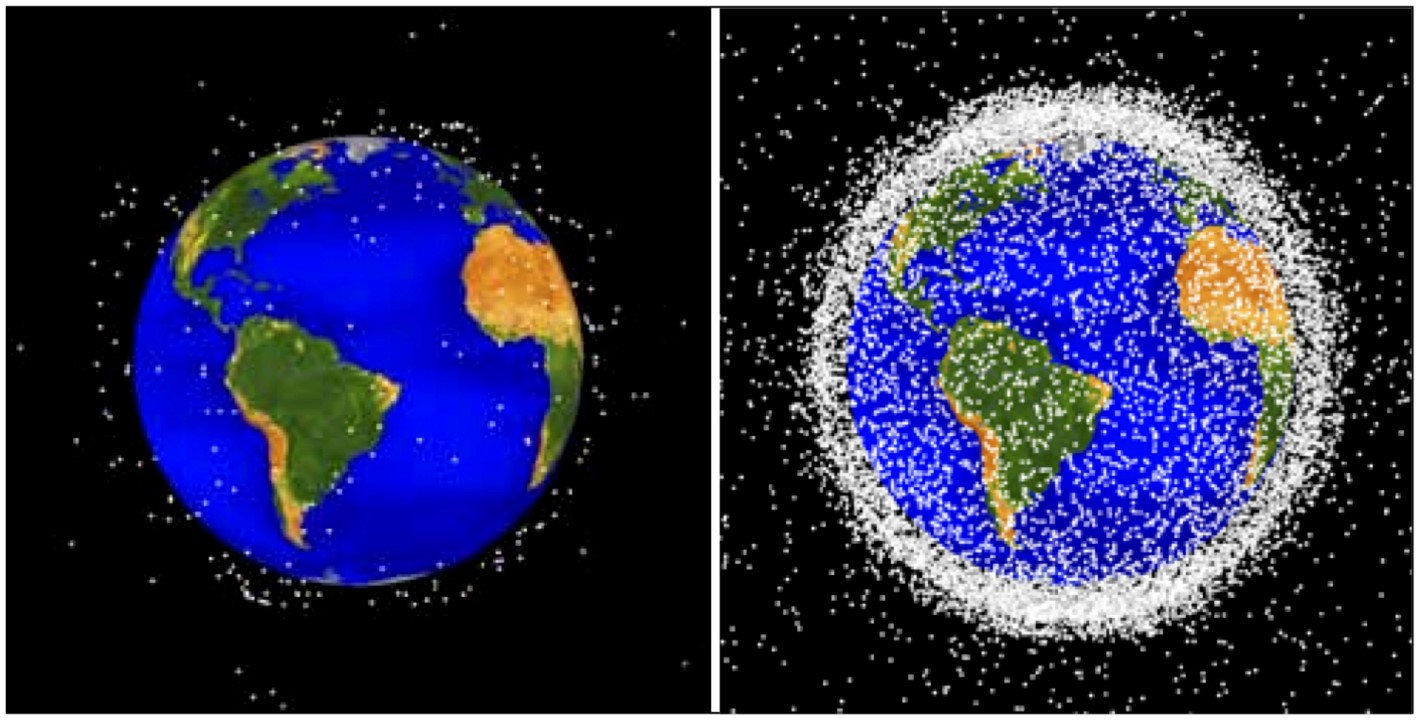
\includegraphics[width=0.75\textwidth]{fig/motivation/TrackedSpaceDebris}
\caption{Tracked space debris in 1963 and fifty years later}
\label{moti-TrackedSpaceDebris}
\end{figure}

The Earth is now surrounded by tens of thousands of sizeable chunks of debris orbiting at speeds upwards of 17,000 miles per hour. Add to these larger pieces an estimated hundreds of thousands of sub-centimeter-sized artificial particles, and you have got a recipe for potential disaster-for while these small particles may not seem imposing, they can present a serious threat to functional spacecraft.


Active Debris Removal (ADR) is necessary to stabilise the growth of space debris, but even more important is that any newly launched objects comply with post-mission disposal guidelines – especially orbital decay in less than 25 years. If this were not the case, most of the required ADR effort would go to compensate for the non-compliance of new objects.\\

Some actively removing space debris ideas or concepts has been proposed by the researchers and institutions around the world. Japan Aerospace Exploration Agency (JAXA), Euorpean Space Agency and Texas A\&M University each presents its own plan.

\newpage

